\section{Materiais e Métodos} \label{methods}

% deve
% • ser elaborada de acordo com as especificidades da pesquisa realizada
% • de modo geral, este parte deve:
% a) descrever o tipo de pesquisa que foi realizada;
% b) narrar as etapas da pesquisa na ordem cronológica dos seus acontecimentos;
% c) anunciar os métodos, técnicas e instrumentos de coleta empregados, como também os critérios de seleção do universo e da amostra pesquisada;
% d) informar minuciosamente o delineamento experimental da pesquisa;
% e) descrever como se deu a coleta de dados e o tipo de coleta que foi realizada;

\subsection{Problemas}

\subsubsection{Acesso à informações}

Foi identificado um problema de acesso à certas atividades em um fluxo de trabalho com muitas repetições por parte de médicos em sistemas LIMS. Com isso, foi elaborado uma maneira de trocar a ordem dos BPMs para maior facilidade de acesso direto à atividade desejada sem a perda de informações.

Para isso, precisamos trocar a ordem do BPM sem perder os dados da atividade, já que a própria transição entre atividades pode significar algum tipo de informação por si só (exemplo: um experimento só deve ser realizado após um outro experimento)

BPMs podem ter múltiplas atividades iniciais e múltiplas atividades finais \cite{Dijkman2008}. Utilizando desse conceito, o workflow a ser alterado foi dividido em duas partes (figura \ref{fig:realWorkflow}): 

\begin{itemize}
    \item Um evento inicial que aponta para a atividade desejada pelo usuário
    \item Um evento inicial que aponta para a atividade inicial do workflow, preenchido até a atividade escolhida para ser a nova primeira atividade inicial
\end{itemize}

\begin{figure}
    \centering
    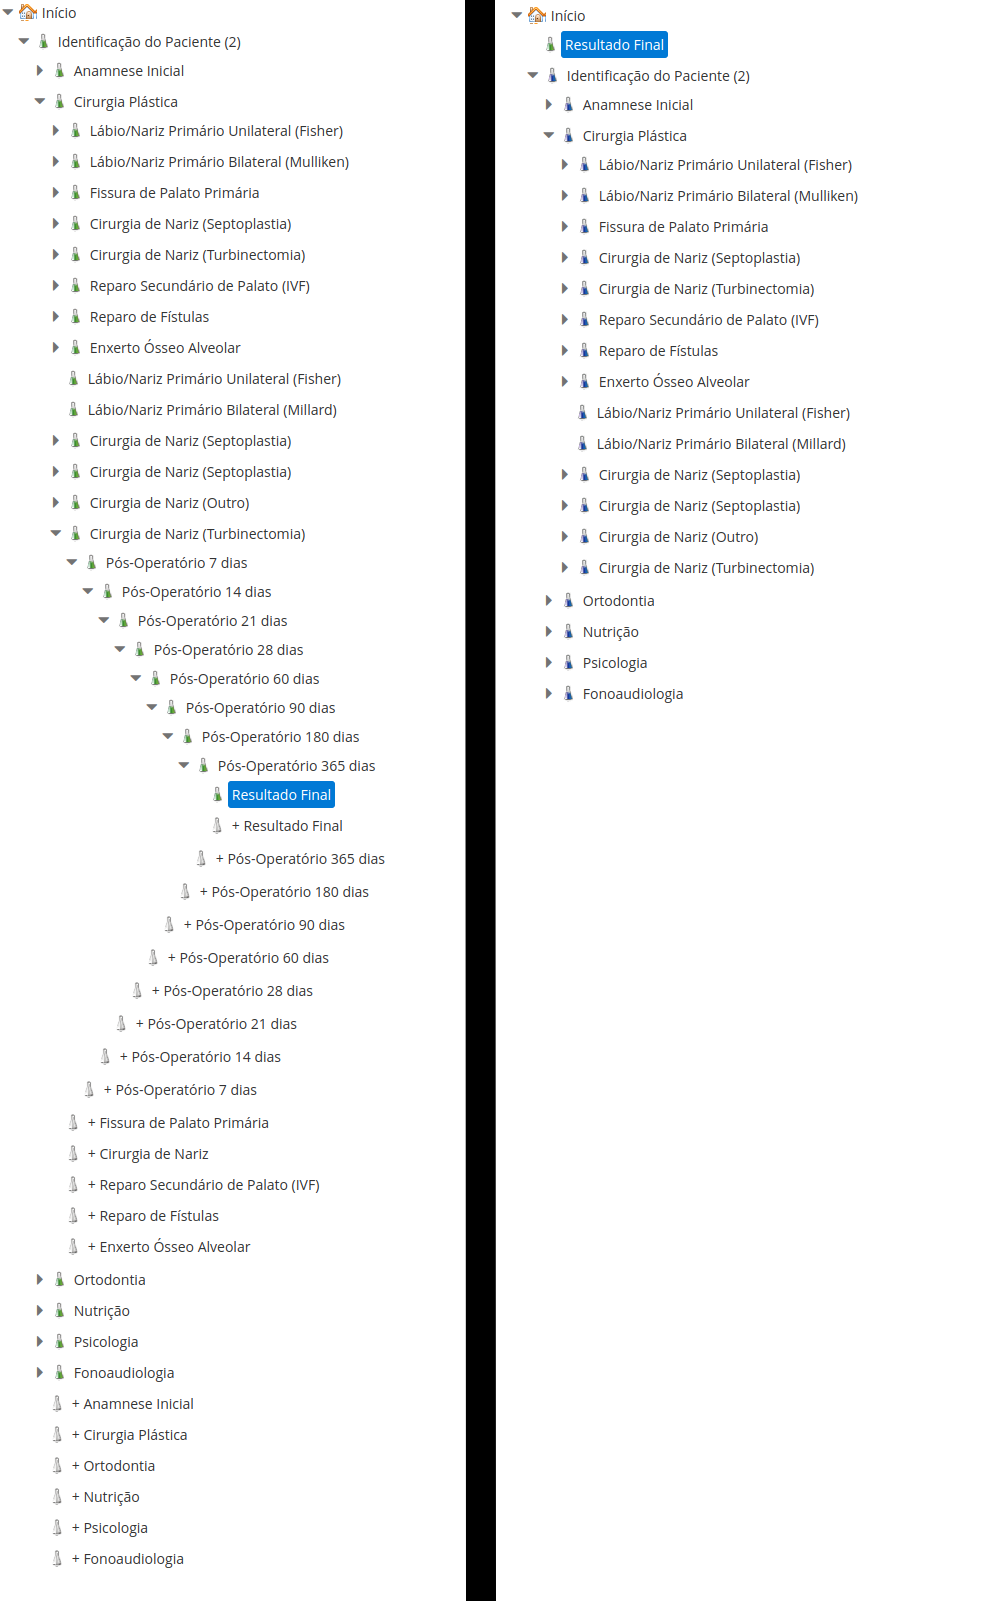
\includegraphics[width=10cm,height=15cm]{imgs/CENTRARE/arvoreNormalEAlterada.png}
    \caption{Workflow com árvore de atividades original à esquerda e workflow com árvore de atividades alterada à direita.}
    \label{fig:realWorkflow}
\end{figure}

Assim, ficam duas atividades iniciais: a primeira com a atividade que o usuário deseja preencher e continuar com seus trabalhos, e a segunda com o workflow original, contendo todas as informações necessárias para o preenchimento da atividade escolhida.

\subsection{Coleta dos dados Dados}

Foi utilizado o LIMS Flux, um LIMS generalizado que pode implementar fluxos de diversos laboratórios com uma interface gráfica presente dentro do próprio sistema \cite{Melo2010}. O Flux é uma ferramenta criada na linguagem Java, utilizando JavaServer Faces como framework de Front-end. O servidor utilizado para deploy é o Apache Tomcat.

Nele, utilizamos dados coletados de três workflows: O workflow BPL - Equipamentos, BPL - POP e o workflow CENTRARE. Os workflows BPL - Equipamentos e BPL - POP servem para controle de equipamentos e registro de informações sobre os procedimentos usados no laboratório, respectivamente, enquanto que o CENTRARE é um workflow para acompanhamento de pacientes com fissura de palato, desde o nascimento até os 20 anos, feito em conjunto com o hospital da baleia em Belo Horizonte.

Os workflows na ferramenta Flux seguem a notação de BPMs (BPMN - Business Process Model Notation) para representar os workflows implementados. Com isso, foi possível testar nesta ferramenta a troca de atividades iniciais e seu impacto nos trabalhos feitos pelo laboratório e fazer a prova de conceito sobre a alteração do fluxo de trabalho em BPMs.

Para o BPL (figura \ref{fig:bplEstrutura}), temos muitos usuários utilizando o mesmo workflow. Mas como o workflow é pouco profundo, com duas até no máximo cinco atividades de profundidade e com maior número de instâncias (ou seja, várias repetições da atividade inicial) ao invés de repetição de atividades dentro do workflow, temos que a centralização em algum atividade específica pode ajudar, mas não é muito necessária.

\begin{figure}
    \centering
    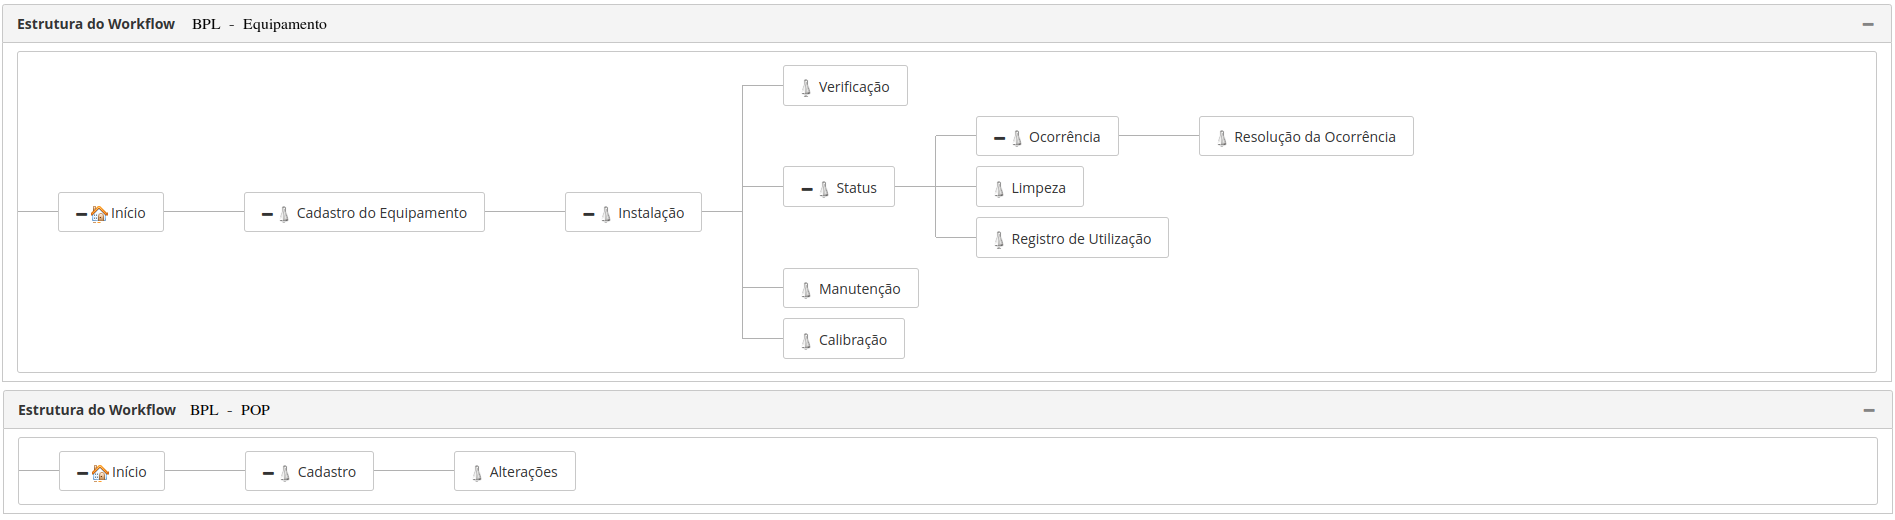
\includegraphics[width=1\textwidth]{imgs/BPL/estrutura.png}
    \caption{Estrutura dos workflows BPL - Equipamentos (Acima) e BPL - POP (Abaixo)}
    \label{fig:bplEstrutura}
\end{figure}

\subsection{Estrutura de workflows}

Para o CENTRARE (figura \ref{fig:centrareEstrutura}), temos muitos médicos que acompanham pacientes separadamente em vários setores de tratamento como cirurgia de palato, cirurgias odontológica, nutricionistas, psicólogos, fonoaudiólogos, entre muitos outros, e todas essas informações ficam em uma instância de um paciente em específico. Isso faz com que tenhamos muitas informações importantes apenas para pessoas específicas no fluxo de tratamento, com uma profundidade grande de atividades no fluxo de trabalho.

\begin{figure}
    \centering
    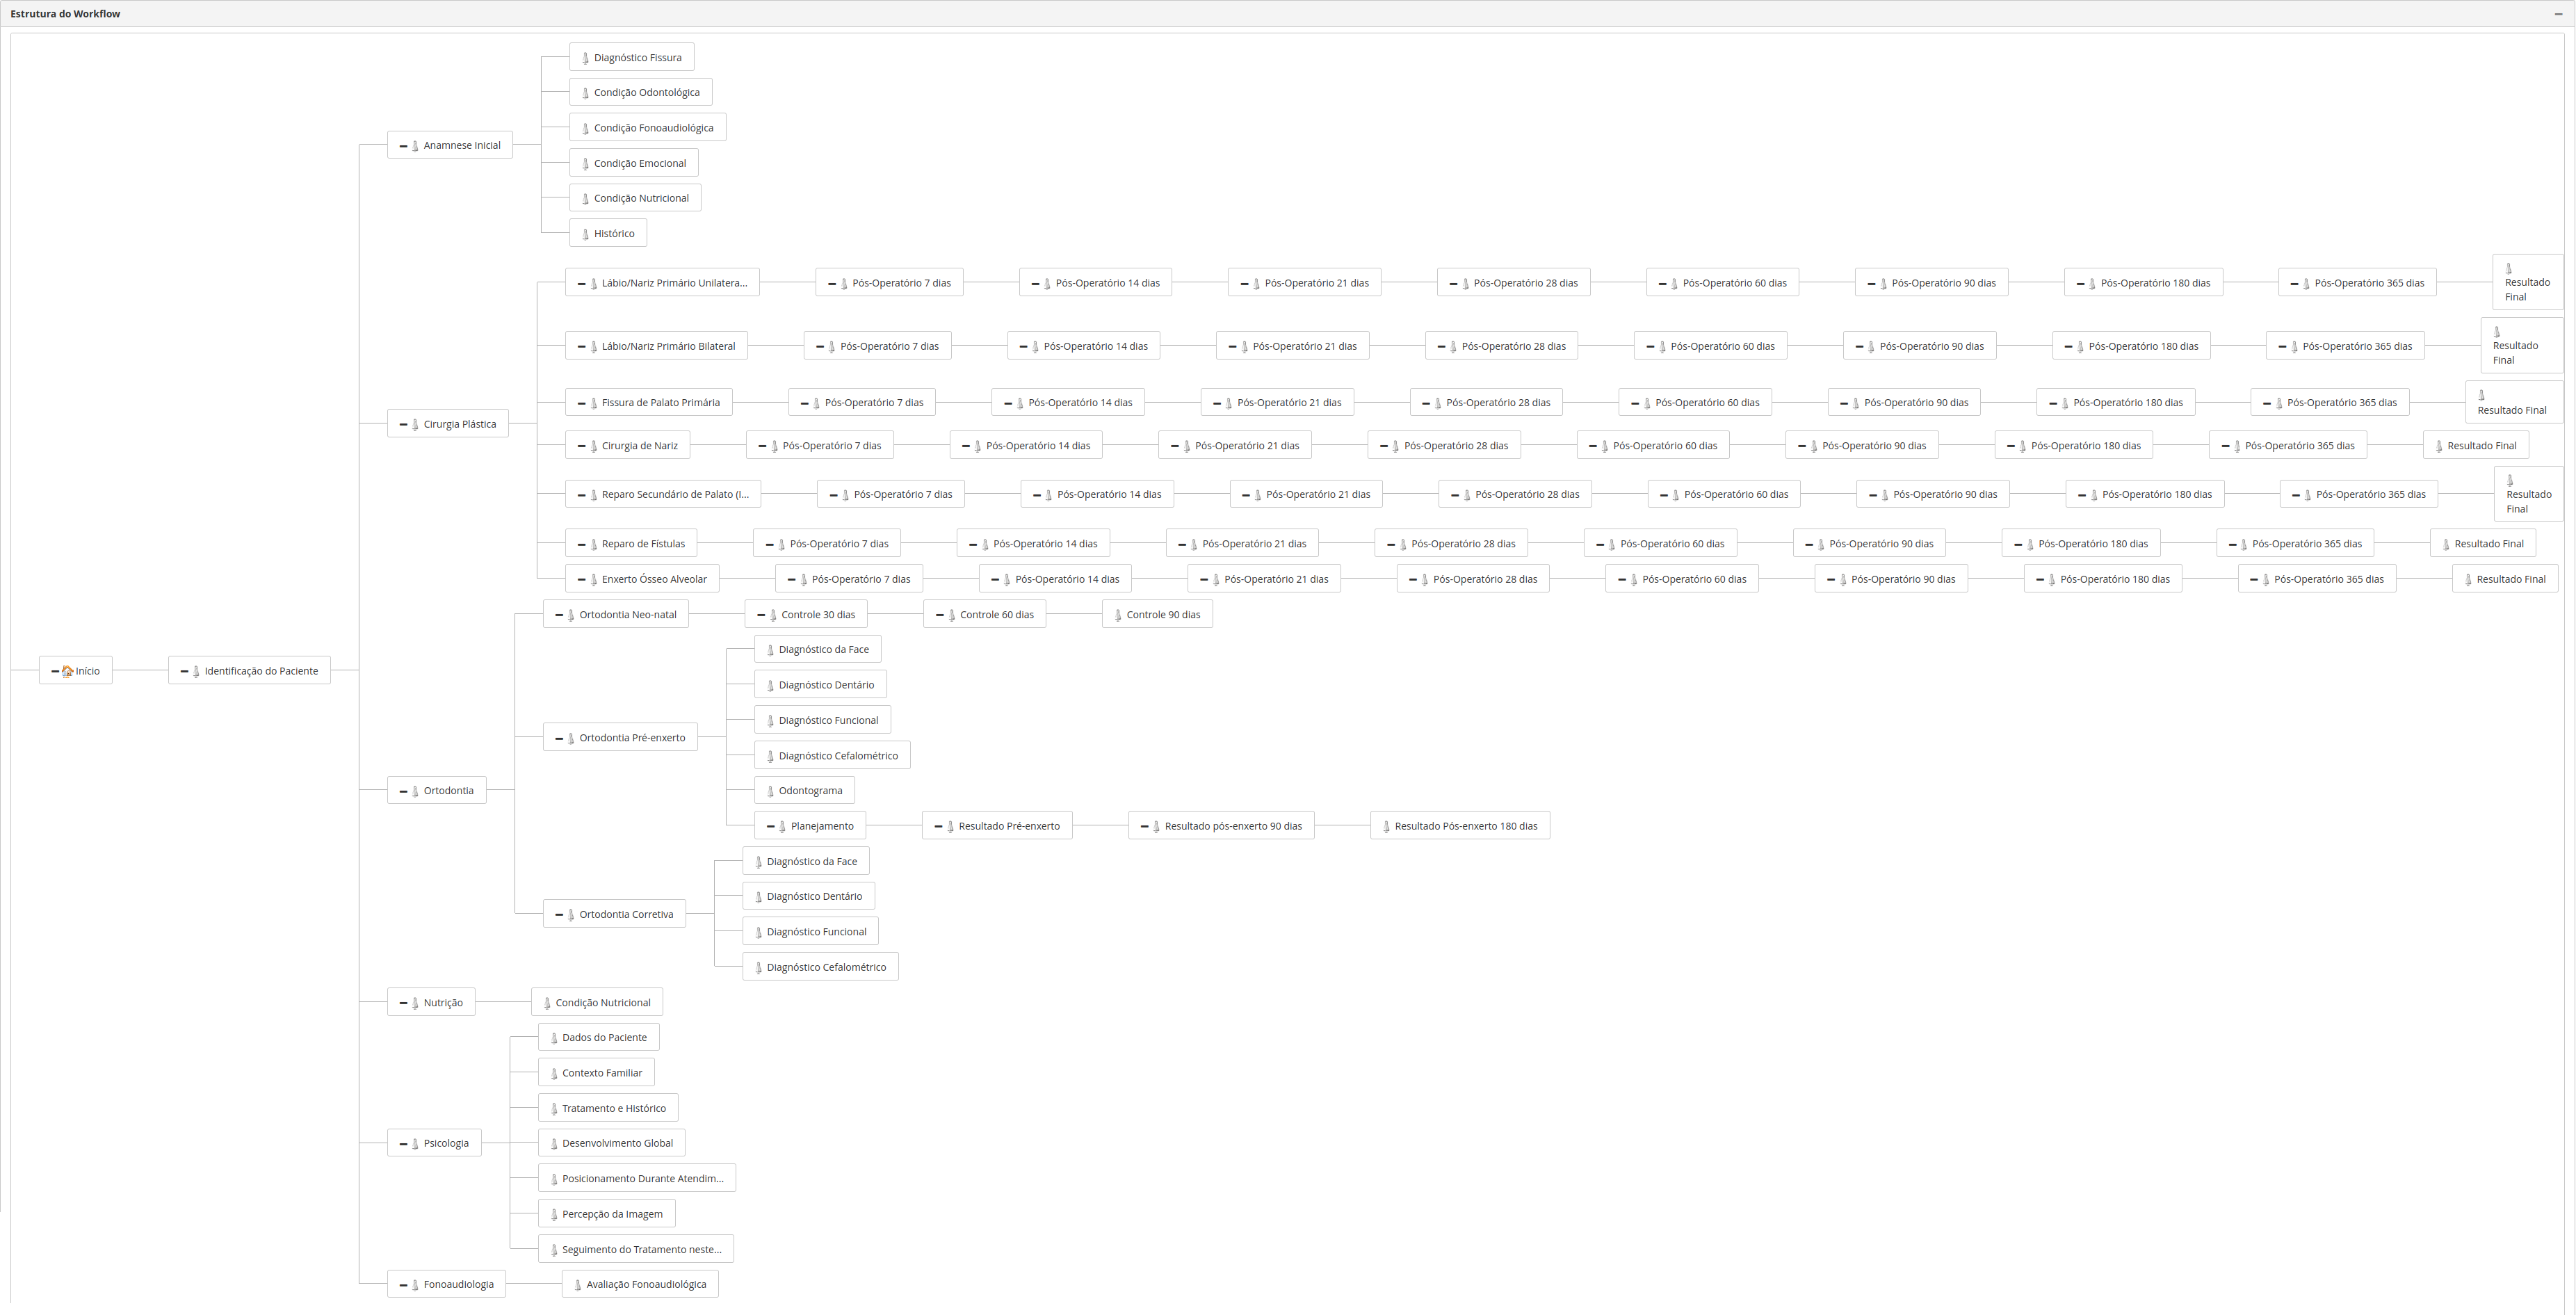
\includegraphics[width=1\textwidth]{imgs/CENTRARE/estrutura.png}
    \caption{Estrutura do workflow CENTRARE}
    \label{fig:centrareEstrutura}
\end{figure}

A centralização de atividades específicas é muito benéfica neste caso: Muitas pessoas trabalhando em partes do fluxo, mesmo que as atividades sejam dependentes de atividades anteriores, já que conseguimos "pular" atividades anteriores que podem não ser tão interessantes para a execução da atividade atual (exemplo: Um diagnóstico feito pelo ortodontista pode não ser interessante para o cardiologista) mas ainda assim obter informações necessárias com o segundo ramo de atividades criado.

Nos workflows BPL, temos dois fluxos que necessitam de compartilhamento de informações, já que um experimento não pode ser realizado se algum equipamento não for calibrado. Como não são as mesmas pessoas que trabalham no mesmo workflow (o técnico dos equipamentos não faz o experimento), com a implementação de BPMs atuais, não é possível que o cientista obtenha essa informação sem pesquisar no outro fluxo de trabalho para encontrar a informação requerida.

Com isso, o compartilhamento de atividades entre BPMs para obtenção de informações ajudaria os cientistas e técnicos a automatizar o envio de emails quando uma atividade se tornasse disponível após uma calibração, o compartilhamento de informações onde um cientista pode dar a informação que um equipamento necessita de reparos ou o técnico pode obter informações de quantos experimentos já foram feitos em um determinado período de tempo em alguma máquina.

Como exemplo de outros workflows que são melhorados com o compartilhamento de atividades são workflows de telemedicina, onde compartilhamento de informações entre pacientes e entre profissionais de saúde é de extrema importância. Também pode ser compartilhado informações administrativas do hospital, tendo informação de quais leitos estão disponíveis, quais produtos (como soros ou remédios) estão disponíveis para uso e quantos médicos estão disponíveis no momento para determinada função.

Também é importante ter o compartilhamento de mensagens entre workflows de biomedicina em laboratórios, em que o compartilhamento de informações entre experimentos ajuda tanto para armazenamento de produtos quanto para os resultados que são importantes para administradores, técnicos de equipamentos e também para outros cientista que estão realizando outros experimentos. Com o compartilhamento de atividades, o administrador do laboratório pode ver quantos experimentos foram realizados em determinada data, informar técnicos que determinado equipamento necessita de manutenção e fazer controle de estoque de itens necessários para o funcionamento correto do local.

\subsection{Implementação}

A implementação de centralização de atividades já foi realizada, começando em otimizações e preparação do sistema Flux. A implementação de compartilhamento de atividades entre workflows estão sendo realizadas e será finalizada até a defesa do mestrado.

Como este recurso requere muitas alterações para adaptação do LIMS Flux, além de várias iterações para chegarmos a uma implementação que faz sentido para o compartilhamento de atividades - como exemplo, existem workflows hospitalares que atividades compartilhadas entre médicos e administradores devem ser vistas apenas pelo administrador, ao invés de todas as atividades administrativas ficarem disponíveis para todos os médicos - este recurso está sendo implementado no momento e ficará pronto até a defesa do mestrado.